% Exercises: pgfplots axes, addplot with expressions and inline tables, legends, groupplots-free layout, log axes.
\documentclass{article}
\usepackage{pgfplots}\pgfplotsset{compat=1.17}
\begin{document}
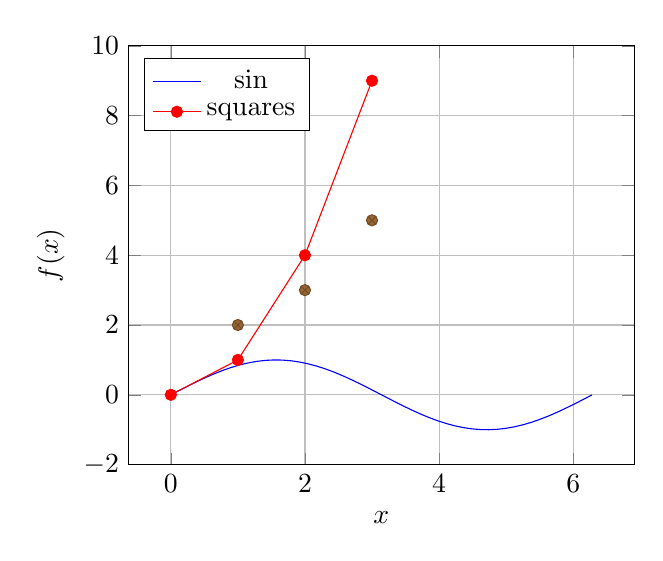
\begin{tikzpicture}\begin{axis}[xlabel=$x$,ylabel=$f(x)$,legend pos=north west,grid=major,width=8cm]
\addplot[blue,domain=0:6.28,samples=50]{sin(deg(x))};\addlegendentry{$\sin$}
\addplot[red,mark=*]table[row sep=\\]{x y\\0 0\\1 1\\2 4\\3 9\\};\addlegendentry{squares}
\addplot+[only marks]coordinates{(1,2)(2,3)(3,5)};\end{axis}\end{tikzpicture}
\begin{tikzpicture}\begin{semilogyaxis}[xmin=0,xmax=10]\addplot[domain=0:10,samples=30]{exp(x)};\end{semilogyaxis}\end{tikzpicture}
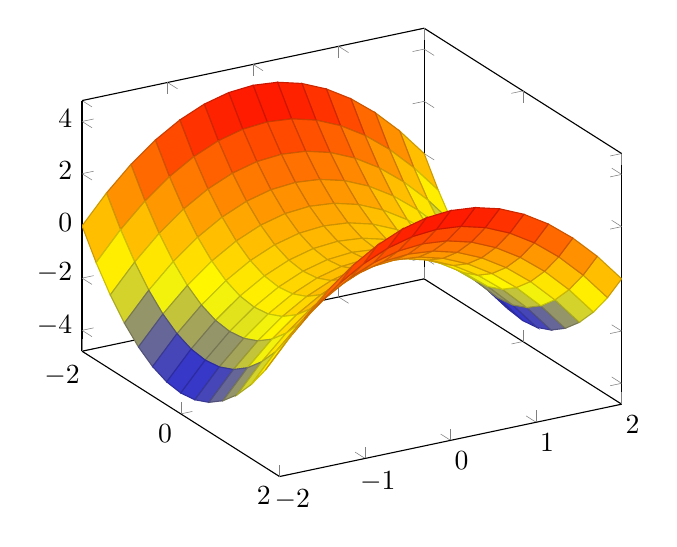
\begin{tikzpicture}\begin{axis}[view={60}{30}]\addplot3[surf,domain=-2:2,samples=15]{x*x-y*y};\end{axis}\end{tikzpicture}
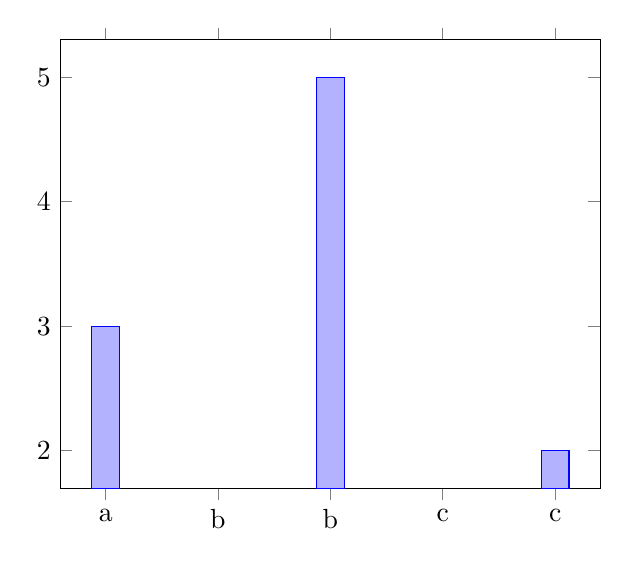
\begin{tikzpicture}\begin{axis}[ybar,symbolic x coords={a,b,c}]\addplot coordinates{(a,3)(b,5)(c,2)};\end{axis}\end{tikzpicture}
\end{document}
